\documentclass[12pt,a4paper]{report}
\usepackage[hmargin=3cm,vmargin=3cm]{geometry}
\usepackage{graphicx}
\usepackage{caption}
\usepackage{array}
\usepackage{listings}
\usepackage{hyperref}
\usepackage{mathtools}
\usepackage{textcomp}
\usepackage{float}
\graphicspath{Images}
\begin{document}
\begin{figure}
\centering

\includegraphics[width = 0.3\textwidth]{iit.png}
\hspace{1cm}

\includegraphics[width = 0.4\textwidth]{fossee-logo.png}
\end{figure}

\title{\textbf{\textbf{Summer Fellowship Report}}\vspace{5mm} \\\small On \\\vspace{5mm} \textbf{\large Spice Simulations using Kicad nightly builds}\vspace{5mm} \\ \vspace{5mm}\small Submitted by\\  \vspace{5mm}  \large \textbf{Akshay NH  and Athul MS}\\ \vspace{5mm}
\small Under the guidance of \\ \vspace{5mm}
\large \textbf{Prof.Kannan M. Moudgalya} \vspace{1mm}\\ Chemical Engineering Department  \vspace{1mm} \\IIT Bombay
}
\vspace{1cm}

\maketitle


\newpage
\title{\textbf{\textbf{\LARGE 
\begin{flushleft}
\textbf{Acknowledgment}
\end{flushleft}
}}}
\large We are extremely thankful to Prof . Kannan Moudgalya for guiding and motivating us throughout the FOSSEE fellowship programme.We would also like to thank our mentors Mrs.Gloria Nandihal and Mr.Athul George for their immense support and advice.Moreover, we are grateful to our fellow friends Mudit Joshi and Ashutosh Gangwar for assisting us with their programming knowledge.Lastly,we extend our warm gratiutude to the managers and staff of FOSSEE for their co-operation and assistance.

\tableofcontents

\chapter{\textbf{Introduction}}
\section{Introduction}
KiCad is an open-source software tool for the creation of electronic schematic diagrams and PCB artwork.KiCad can be considered mature enough to be used for the successful development and maintenance of complex electronic boards.KiCad does not present any board-size limitation and it can easily handle up to 32 copper layers, up to 14 technical layers and up to 4 auxiliary layers. KiCad can create all the files necessary for building printed boards, Gerber files for photo-plotters, drilling files, component location files and a lot more.Being open source (GPL licensed), KiCad represents the ideal tool for projects oriented towards the creation of electronic hardware with an open-source flavour.

Stable builds
Stable releases of KiCad can be found in most distribution’s package managers as kicad and kicad-doc. If your distribution does not provide latest stable version, please follow the instruction for unstable builds and select and install the latest stable version.

Unstable (nightly development) builds
Unstable builds are built from the most recent source code. They can
sometimes have bugs that cause file corruption, generate bad gerbers, etc, but are generally stable and have the latest  features.

\chapter{\textbf{Structure of the Signal Processing toolbox}}
The toolbox has two types of files:
\section{Visible Files}
\begin{itemize}
\item loader.sce
\item builder.sce
\item demos
\item etc
\item jar
\item cleaner.sce
\item testfile.sce
\item unloader.sce
\item README.md
\item help
\end{itemize}

The primary step that one has to do, to use this toolbox for the first time is that , one has to essentially go through the README.md file of the toolbox. This file has the text providing the guidance on how to use the toolbox.  

\subsection{loader.sce}
It’s basically a file that calls for the function FOSSEE\textunderscore Signal\textunderscore processing\textunderscore toolbox.start present in the etc folder. This has to be executed first on opening the toolbox, using the command \char`\"exec loader.sce\char`\".
in the scilab console.


\subsection{builder.sce}
This file builds the macros,help and the loader.sce files. Type the command \char`\"exec builder.sce\char`\" in the scilab console to execute this file.\\
Both these have to executed every time, to load the toolbox for usage.

\subsection{demos}
This folder includes the examples taken from  \url{https://in.mathworks.com/help/signal/examples/dft-estimation-with-the-goertzel-algorithm.html }, which is function used for DFT Estimation with the Goertzel Algorithm.

\subsection{macros}
It’s the main folder of the toolbox, which has all the signal processing functions of the toolbox.

\subsection{etc}
Its a folder which consists of FOSSEE\textunderscore Signal\textunderscore processing\textunderscore toolbox.start and FOSSEE\textunderscore Signal\textunderscore processing\textunderscore toolbox.quit files.
These files are used to start and exit files of the toolbox.

.start file
It will run a script when loader.sce is run from root toolbox directory. It will run loader files in all of the directories and link to important library.

.quit file
It will run a script when unloader.sce is run from root toolbox directory. It will unlink all of the important libraries.


\subsection{jar}
This folder has scilab\textunderscore en\textunderscore US.jar file. This file is basically a Java Archive package file format typically used to aggregate many Java class files and associated metadata and resources (text,images etc.) into a file for distribution.

\subsection{cleaner.sce}
This file is generated by builder.sce. On executing this file, we actually delete the loader.sce and the unloader.sce files.
One caution to the users is that  \textbf{do not edit this file.}

\subsection{testfile.sce}
This file is used to validate all the functions present in the toolbox macros. This file is executed in the Travis CI (Continuous Integration).

\subsection{unloader}
It unloads the toolbox.

\subsection{help}
It contains the help files of all the functions present in the toolbox(macros) as .xml files.

\section{Hidden Files}
These files have to included in the git repository before pushing it to the github. To view these files in the git repository use the command:  \\
\char`\"ls -a\char`\"   on the terminal in the git repository directory.  


\begin{itemize}
\item .gitignore 
\item .travis.yml
\end{itemize}

\subsection{.gitignore}
This file enables the user to explicitly tell git to ignore certain files. In our toolbox, we have included just a statement  \char`\" \char`\* \char`\~ \char`\" , indicating that all the file names having the sign \char`\"\char`\~\char`\" (\char`\"tilde\char`\") in the end(or suffixed) are ignored by git (when intentionally gone untracked).  

\subsection{.travis.yml}
This file is included to facilitate the builds we can trigger in Travis CI. \\
Travis CI actually provides a default build environment and a default set of steps for each programming language. We can customize any step in this process in .travis.yml. Travis CI uses .travis.yml file in the root of our repository to learn about our project and how we want our builds to be executed. .travis.yml can be very minimalistic or have a lot of customization in it.

\begin{figure}[H]
\centering
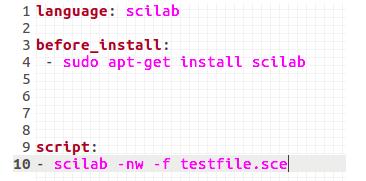
\includegraphics[width = 0.5\textwidth]{travisyml.png}
\captionof{figure}{ .travis.yml file}
\end{figure}

The above figure shows the different sections involved in the .travis.yml file.\\
So each time when a build is triggered by the user, tracis engine actually downloads scilab (as per before\textunderscore install section) and then a new scilab instance is opened in the terminal without any gui (-nw flag) and executes testfile.sce in the toolbox ( because of the -f flag used here).


\newpage
\title{\textbf{\textbf{\LARGE 
\begin{flushleft}
\textbf{Reference}
\end{flushleft}
}}}




\begin{itemize}
\item \url{http://docs.kicad-pcb.org/stable/en/getting_started_in_kicad.pdf}
\item \url{https://github.com/KiCad/kicad-source-mirror}
\item  \url{https://github.com/FOSSEE/eSIm-Kicad-Simulations}
\item \url{ https://forum.kicad.info/}
\item \url{ http://www.ecircuitcenter.com/Basics.htm}
\item \url{http://www.ecircuitcenter.com/SPICEsummary.htm}
\end{itemize}
\end{document}



